%- HandOut Flag -----------------------------------------------------------------------------------------
\newif\ifHandout

%- D0cum3nt ----------------------------------------------------------------------------------------------
\documentclass[beamer,10pt]{standalone}   
%\documentclass[beamer,10pt,handout]{standalone}  \Handouttrue  

%- HandOut Flag -----------------------------------------------------------------------------------------
\ifHandout
	\setbeameroption{show notes} %print notes   
\fi

	
%- Packages ----------------------------------------------------------------------------------------------
\usepackage{custom-style}
\usetikzlibrary{positioning}
\usepackage{multicol}


%--Beamer Style-----------------------------------------------------------------------------------------------
\usetheme{toninus}
\usepackage{animate}
\usetikzlibrary{positioning, arrows}
\usetikzlibrary{shapes}

\begin{document}
%-------------------------------------------------------------------------------------------------------------------------------------------------
\begin{frame}{Phase Space via Configuration Space}
	\begin{itemize}
	\item To introduce the notion of {\bf phase space} it is useful to start from the auxiliary concept of {\bf configuration space}.
	\end{itemize}

	\vfill
	\begin{itemize}
		\item<2-> this notion is based on three \emph{primitive concepts}:
	\end{itemize}
	\onslide<2->{
		\begin{center}
			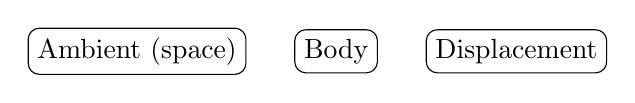
\begin{tikzpicture}[>=stealth,every node/.style={shape=rectangle,draw,rounded corners},node distance=0.05\linewidth,]
		    % create the nodes
			    \node[] (a1) {Ambient (space)}; %Physical space
			    \node[] (a2)[right =of a1] {Body}; %(Physical) system
			    \node[] (a3)[right =of a2] {Displacement}; %configuration
			\end{tikzpicture}
		\end{center}
	}
\end{frame}
\note[itemize]{
	\item In molte presentazioni di nozioni matematiche per concetto primitivo o nozione primitiva si intende un concetto che, per la propria semplicità ed intuitività, si rinuncia a definire mediante termini e concetti già definiti all'interno di un sistema formale, e che al contrario si sceglie di sfruttare per formulare la definizione di altri concetti; pertanto un concetto primitivo si accetta senza spiegazioni perché il suo significato è ovvio.
}
%-------------------------------------------------------------------------------------------------------------------------------------------------


%-------------------------------------------------------------------------------------------------------------------------------------------------
\begin{frame}[t]{Configuration Space: the Ambient}
	\begin{center}
		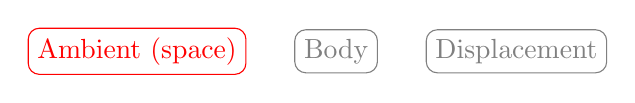
\begin{tikzpicture}[>=stealth,every node/.style={shape=rectangle,draw,rounded corners},node distance=0.05\linewidth,]
	    % create the nodes
		    \node[red] (a1) {Ambient (space)}; %Physical space
		    \node[gray] (a2)[right =of a1] {Body}; %(Physical) system
		    \node[gray] (a3)[right =of a2] {Displacement}; %configuration
		\end{tikzpicture}	
	\end{center}
	\begin{columns}
		\begin{column}[T]{0.5\textwidth}
			\begin{itemize}
				\item The physical space, our universe.
				\item It is the stage on which the act of dynamics takes place.
			\end{itemize}
			\vspace{1em}
			\onslide<2->{					
				\begin{exblock}
					Consider a laboratory.
				\end{exblock}
			}
			\vspace{1em}
			\onslide<3->{
				\begin{mathblock}
					is the Euclidean space $E=\mathbb{R}^3$.
					\\				
					(fixed a \emph{Galilean observer}) 
				\end{mathblock}
			}		
		\end{column}
		\begin{column}[T]{0.5\textwidth}
			\onslide<2->{
				\begin{center}
					\includegraphics[width=\textwidth]{Pictures/emptylab}
				\end{center}
			}
		\end{column}
	\end{columns}
\end{frame}
\note[itemize]{
	\item
}
%-------------------------------------------------------------------------------------------------------------------------------------------------


%-------------------------------------------------------------------------------------------------------------------------------------------------
\begin{frame}[t]{Configuration Space: the Body}
	\begin{center}
		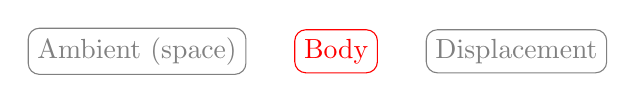
\begin{tikzpicture}[>=stealth,every node/.style={shape=rectangle,draw,rounded corners},node distance=0.05\linewidth,]
	    % create the nodes
		    \node[gray] (a1) {Ambient (space)}; %Physical space
		    \node[red] (a2)[right =of a1] {Body}; %(Physical) system
		    \node[gray] (a3)[right =of a2] {Displacement}; %configuration
		\end{tikzpicture}
	\end{center}

	\begin{columns}
		\begin{column}[T]{0.5\textwidth}
			\begin{itemize}
				\item it is a bulk of matter, a portion of the ambient, we wish to study.
			\end{itemize}
								
			\vspace{1em}
			\only<2->{			
				\begin{exblock}
					Consider the bob of a rigid pendulum.
				\end{exblock}
			}

			\vspace{1em}
			\only<3->{
				\begin{mathblock}
					\begin{columns}
						\begin{column}{0.025\textwidth}
						\end{column}
						\begin{column}[T]{0.5\textwidth}
							is a submanifold $B\hookrightarrow E$ with boundary
							\vspace{-.5em}
							\begin{center}
								\includegraphics[width=.25\textwidth]{Pictures/bob}
							\end{center}
						\end{column}					
						\begin{column}[T]{0.45\textwidth}
							is a point in $B\in E$ (the center of mass).
							\begin{center}
								\tikz[] \node[scale=0.5,coordinate,fill=red,circle] (n1) {};	
							\end{center}						
						\end{column}							
					\end{columns}
					\begin{column}{0.025\textwidth}
					\end{column}
				\end{mathblock}
			}
			\vfill
%			\only<4->{
%				\begin{bracketbox}%{Key point:}
%					\small
%					Remind:
%					The ambient acts on the body via \emph{forces} and \emph{constraints}.
%				\end{bracketbox}
%			}	
		\end{column}
		\begin{column}[T]{0.5\textwidth}
				\begin{center}
					\includegraphics<1>[width=\textwidth]{Pictures/emptylab}
					\includegraphics<2->[width=\textwidth]{Pictures/Pendolab}					
				\end{center}
		\end{column}
	\end{columns}
\end{frame}
\note[itemize]{
	\item "è il protagonista della recita"
	\item remind the implied idea: 	The ambient acts on the body via \emph{forces} and \emph{constraints}.
}	
%-------------------------------------------------------------------------------------------------------------------------------------------------


%-------------------------------------------------------------------------------------------------------------------------------------------------
\begin{frame}[t]{Configuration Space: the displacement}
	\begin{center}
		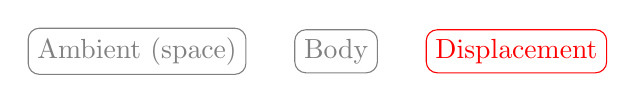
\begin{tikzpicture}[>=stealth,every node/.style={shape=rectangle,draw,rounded corners},node distance=0.05\linewidth,]
	    % create the nodes
		    \node[gray] (a1) {Ambient (space)}; %Physical space
		    \node[gray] (a2)[right =of a1] {Body}; %(Physical) system
		    \node[red] (a3)[right =of a2] {Displacement}; %configuration
		\end{tikzpicture}
	\end{center}

	\begin{columns}
		\begin{column}[T]{0.5\textwidth}
			\begin{itemize}
				\item is how the body is placed inside the space.
				\item configuration (spatial displacement) of the physical system admissible by the constraints.
			\end{itemize}
			\vspace{1em}
			\only<2->{
				\begin{exblock}[Pendulum]
					one of the possible positions where the bob can be placed allowed by the rod.		
				\end{exblock}
			}	
			\vspace{1em}
			\only<3->{
				\begin{mathblock}
					is a (smooth) function $B \to E$.				
				\end{mathblock}
			}					
			
		\end{column}
		\begin{column}[T]{0.5\textwidth}
			\begin{center}
				\includegraphics<1>[width=\textwidth]{Pictures/Pendolab}
				\only<2->{	
					\animategraphics[autoplay,palindrome,width=\textwidth]{5}{Pictures/pendolum-frame/pendo}{1}{9}
				}
			\end{center}
		\end{column}
	\end{columns}
\end{frame}
\note[itemize]{
	\item
}

%-------------------------------------------------------------------------------------------------------------------------------------------------

%-------------------------------------------------------------------------------------------------------------------------------------------------
\begin{frame}[t]{Configuration Space}
	%	
	\center
	\begin{zigzagbox}
		Neglect the fluff $\quad\rightsquigarrow\quad$ abstract (synthetic) mathematical setting
	\end{zigzagbox}
	
	\begin{columns}
		\begin{column}[T]{0.5\textwidth}
			\begin{itemize}
				\item<2-> Consider the set $Q$  of all the possible displacements (spatial configurations).
			\end{itemize}
			%			
			\vspace{1em}
			\onslide<3->{
				\begin{exblock}[Pendulum]
					$Q$ = 
						the locus of points on the plane with fixed distance from the pivot (the circle $S^1$).	
				\end{exblock}
			
			}			
			%			
			\vspace{1em}
			\onslide<4->{
				\alert{Upshot: $Q$ is a smooth manifold}
							
			\begin{defblock}[Configuration Space]
				Smooth manifold of all the system configurations admissible by the constraints.
			\end{defblock}			
			}
		\end{column}


		\begin{column}[T]{0.5\textwidth}
			\begin{center}
			\only<1>{				
				\resizebox{\textwidth}{!}{		
				    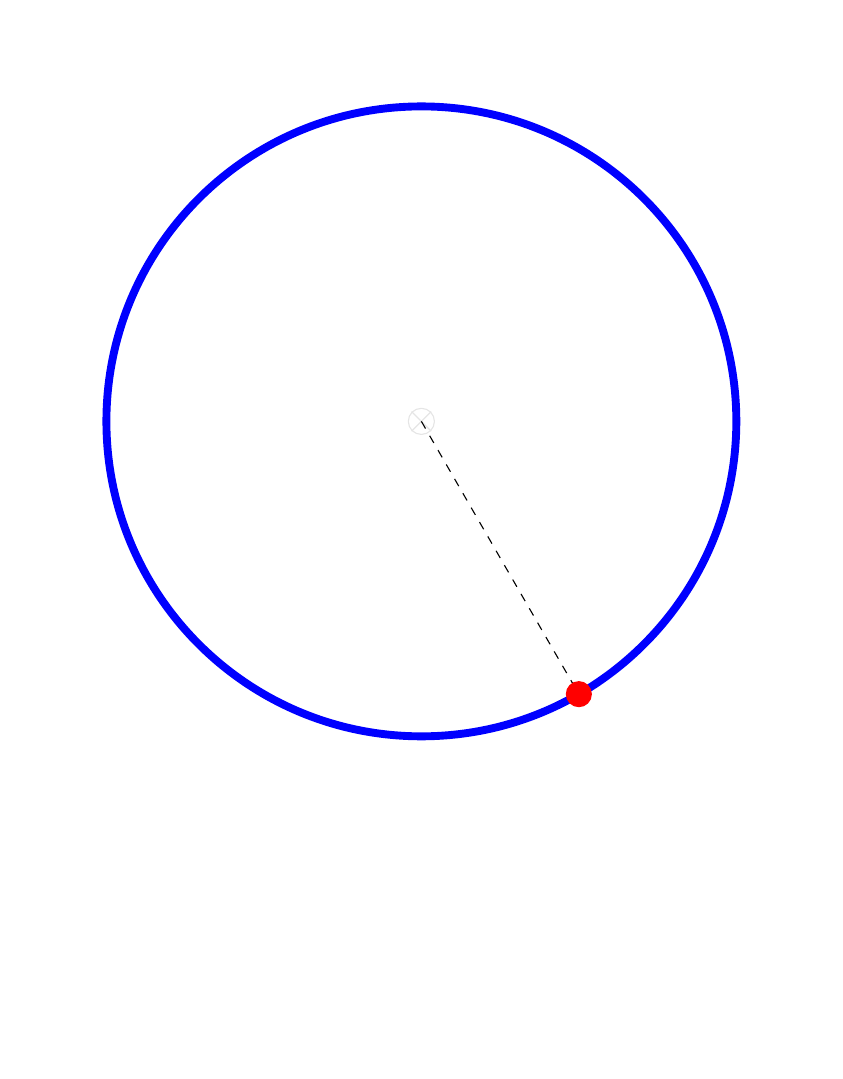
\begin{tikzpicture}
					    %frame
					    \draw[draw=none] (-5,-8) rectangle (5,5);
						% Support
						\coordinate (o) at (0,0);
						\node[cross out,draw,black!10] (0,0){};
						\node[circle,draw,black!10] (0,0){};
						% Bob's trajectory
						\draw[blue,line width=1mm,] (0,0) circle (4);
						% Rod + Bob
						\draw[dashed] (0,0) -- (-60:4) node[fill,circle,red](m){};
				    \end{tikzpicture}
				}
			}
			\only<2->{				
				\resizebox{\textwidth}{!}{		
					\pgfmathtruncatemacro\steps{50}
					\pgfmathtruncatemacro\maxtheta{30}
					\pgfmathtruncatemacro\pi{3.14}
					\begin{animateinline}[autoplay,loop]{10} % 5 fps, same as 0.2 s transduration
					  \multiframe{\steps}{i=0+1}{
					    \begin{tikzpicture}
					    \pgfmathsetmacro\fraction{\i/(\steps-1)}
						\pgfmathsetmacro\theta{\maxtheta*cos(360*\fraction)-90}
					    %frame
					    \draw[draw=none] (-5,-8) rectangle (5,5);
						% Support
						\coordinate (o) at (0,0);
						\node[cross out,draw,black!10] (0,0){};
						\node[circle,draw,black!10] (0,0){};
						% Bob's trajectory
						\draw[blue,line width=1mm] (0,0) circle (4);
						% Rod + Bob
						\draw[dashed] (0,0) -- (\theta:4) node[fill,circle,red](m){};
					    \end{tikzpicture}
					  }
					\end{animateinline}
				}
			}
			\end{center}
		\end{column}
	\end{columns}
\end{frame}
\note[itemize]{
	\item
}
%-------------------------------------------------------------------------------------------------------------------------------------------------

%-------------------------------------------------------------------------------------------------------------------------------------------------
\begin{frame}{Quick reminder: Smooth manifolds}
	\tcbset{colback=white,
	colbacktitle=white,
	colframe=red!70!black,
	boxrule=1pt,
	colupper=red!70!black,
	arc=15pt,
	}
		\begin{columns}[]
		\begin{column}{0.475\textwidth}
			\begin{tcolorbox}[enhanced,frame hidden,borderline={0.5pt}{0pt}{red!70!black}]
			Extrinsically:\\
			\color{black} 
			\emph{higher dimensional} surface 
			\\ smoothly embedded in $\mathbb{R}^N$.
			\\
			\small (for a suitably large $N$).		
			\end{tcolorbox}
	
			\center
			\onslide<2->{
				\includegraphics[width=.9\textwidth, height = 10em]{Pictures/smooth-mfd-Lee} 	
				%\includegraphics[width=.7\textwidth]{Pictures/LocalChart} 		
			}
		\end{column}
		\begin{column}{0.52\textwidth}
			\center
			\includegraphics[width=.5\textwidth]{Pictures/embedded_sphere} 	
			
			\onslide<2->{
				\begin{tcolorbox}[enhanced,frame hidden,borderline={0.5pt}{0pt}{red!70!black}]
					Intrinsically:\\
					\color{black} 
					A topological spaces equipped with 
					\\ (a maximal atlas of compatible) 
					\\
					charts.
				\end{tcolorbox}			
			}			
		\end{column}
		\end{columns}
		
		\vfill
		\begin{columns}[]
			\begin{column}{0.1\textwidth}\end{column}
			\begin{column}{0.6\textwidth}
				\onslide<3->{
			\begin{tcolorbox}[enhanced,frame hidden,borderline={0.5pt}{0pt}{brown!70!black}]
				A reasonably general setting for defining:
				\begin{itemize}
					\item[•] Reference frames / coordinates (observers);
					\item[•] Smoothness.
				\end{itemize}
			\end{tcolorbox}
				}
			\end{column}
			\begin{column}{0.1\textwidth}\end{column}
		\end{columns}






\end{frame}
\note[itemize]{
	\item
}
%-------------------------------------------------------------------------------------------------------------------------------------------------


%-------------------------------------------------------------------------------------------------------------------------------------------------
\begin{frame}[t]{Configuration Space: a slightly more difficult example}
		\center
	\begin{bracketbox}
		Double pendulum.
	\end{bracketbox}
	

	\vfill
	\only<1-3>{
		\begin{columns}[T]
			\begin{column}{0.5\textwidth}
				\begin{center}
					\includegraphics[width=.75\textwidth]{Pictures/bipend-abstract}	
				\end{center}
			\end{column}
			\begin{column}{0.5\textwidth}
				\begin{center}
					\only<1>{
						\noindent Toy model for:
						\begin{center}
							\includegraphics[width=.55\textwidth]{Pictures/robo_arm}
						\end{center}
						mechanical arms.
					}
					\only<2>{
						\noindent Toy model for:
						\begin{center}
							\includegraphics[width=.65\textwidth]{Pictures/amino_acids}
						\end{center}
						Proteins (amino acid chains).	
					
					}
					\only<3>{
						\includegraphics[width=.75\textwidth]{Pictures/bipend-phase}	
					}
				\end{center}
			\end{column}
		\end{columns}	
	}
	\only<4->{
		\animategraphics[autoplay,palindrome,width=\textwidth]{5}{Pictures/lessig-pibend-frame/bipend-}{2}{6}
	}
	\vfill
	\onslide<3->{\center\alert{Configuration space is a Torus}}


\end{frame}
\note[itemize]{
	\item per quanto sia un toy model è il primo passo per modellizzare una proteina. (Catena di amminoacidi posti a distanza pressochè costante fra di loro)
	\item This case (bi-pendulum) examplify how constraints can be enforced intrinsically choosing an appropriate geometric framework. (2-coordinates instead of the 4 x-y coordinates needed to fix the two endopoints.

}
%-------------------------------------------------------------------------------------------------------------------------------------------------

\end{document}